\documentclass[../report.tex]{subfiles}
\begin{document}   

% User manual
\subsection{Software Setup Instructions} \label{ssec:setup_instructions}

For the simple case where no API keys need to be changed, setting up and running UltraCast is as simple as running:

\begin{verbatim}
    # cd to the root directory of the git repo
    ./start.sh
\end{verbatim}
%
This script will: 
\begin{itemize}
    \item Create a python virtual environment (venv) for the backend
    \item Install all required python packages in the venv
    \item Install all npm packages that are required for the frontend
    \item Launch the backend web server (if the --local flag is used)
    \item Launch the frontend
    \item Open UltraCast in your browser (this may not work on VLab)
\end{itemize}

UltraCast can be run using either a local or remote GraphQL endpoint.
The remote GraphQL endpoint is preferred due to lower latency (it must make successive MongoDB database operations which can be slow if network latency is high).
It is highly recommended to run UltraCast in remote mode on UNSW CSE machines as the port used for the GraphQL endpoint is often already in use.

To run UltraCast using a local backend web server:

\begin{verbatim}
    # cd to the root directory of the git repo
    ./start.sh --local
\end{verbatim}

Once the web server is installed and running you will see a message like:

\begin{verbatim}
    Serving frontend at http://localhost:43689/
\end{verbatim}

You can then navigate to UltraCast in a web-browser at the link printed to the terminal e.g. \verb|http://localhost:43689|.
To avoid failing to launch because a port is already in use, the port which is used is decided at runtime. Ensure that you use the correct port.

\subsection{Configuration}

The following external services are used and their IP addresses and/or API keys will need to be set in configuration files:

\begin{itemize}
    \item Algolia
    \item MongoDB Instance (hosted in a cloud container e.g. Amazon EC2)
    \item S3 Bucket
    \item Backend GraphQL endpoint (if not hosted on local machine)
\end{itemize}

Some of these variables need to be set for the frontend and some for the backend.

\subsubsection{Backend Configuration}

The backend is configured by using python files which set various configuration variables. These include options including:
\begin{itemize}
    \item The IP address of the MongoDB instance
    \item The MongoDB database
    \item Flask secret keys (for encryption)
    \item Algolia API key and user
\end{itemize}
A full list of the variables that can be set is in \verb|backend/config/default_settings.py|.
%
Any variables that are not set are defaulted to the value in \verb|backend/config/default_settings.py|.
You can override these settings by writing a new python file and setting the environment variable \verb|ULTRACAST_BACKEND_SETTINGS| to be the real path of this file. 
For example if the settings file is at \verb|~/ultracast_settings.py|, you could do:

\begin{verbatim}
    export ULTRACAST_BACKEND_SETTINGS=$(realpath ~/ultracast_settings.py)
    bash backend/start.sh
\end{verbatim}

\subsubsection{Frontend Configuration}

The frontend can be configured by editing the file \verb|frontend/src/api/config.js| Here you can set options including:
\begin{itemize}
    \item The backend GraphQL endpoint to use
    \item Algolia API key and user
\end{itemize}

\subsection{Logging}

When \verb|./start.sh| or \verb|backend/start_production.sh| are used to launch the backend, by default backend logs will be recorded to \verb|backend/logs.txt|.
This behaviour can be modified by changing the err-log option in \verb|backend/backend_app.py|.
When the backend is run in development mode, logs are printed to the terminal.

Frontend logs can be accessed via the web-browser console.

\newpage

\subsection{Site Usage and Functionality Guide}

\subsubsection{Prerequisites}

Please ensure that:
\begin{itemize}
    \item The site is running (See \cref{ssec:setup_instructions} for help)
    \item Chrome or Firefox is used to improve performance
\end{itemize}

\subsubsection{Login}

Enter \verb|localhost:4000| into your browser to reach the UltraCast
login page as seen in \cref{fig:UM_Login}. After filling in your email and password 
click "SIGN IN" to be redirected to the homepage.
%
\begin{figure}[ht] 
    \centering
    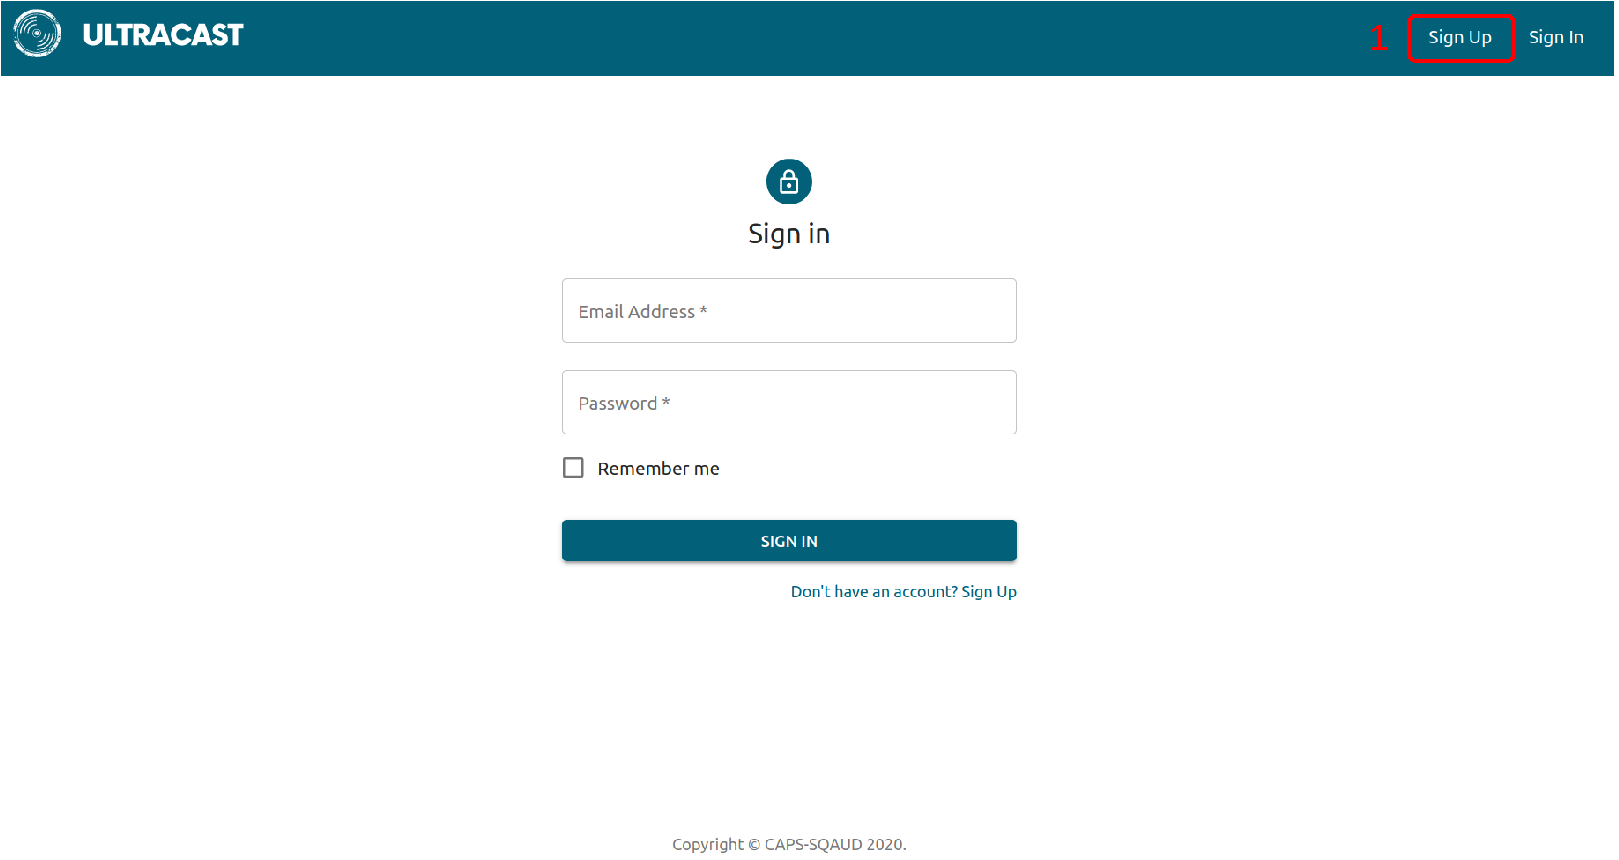
\includegraphics[width=16cm]{resources/UM_Login}
    \caption{UltraCast Login}
    \label{fig:UM_Login} 
\end{figure}

\underline{If you have not already signed up} click on "SIGN UP", labelled with a red "1" in \cref{fig:UM_Login}, where
you will be prompted to fill in your name, email and password before clicking "Sign Up" to login:

\newpage

\subsubsection{Homepage}

After logging in you will be directed to the homepage as seen in \cref{fig:UM_Homepage} below. The 
homepage consists of two components \underline{which will be empty if you are a new user}:
%
\begin{itemize}
    \item \textbf{Recommended Podcasts}: Podcasts our recommended suggests based on your activity
    \item \textbf{Recently Listened}: Podcast Episodes that you have listened to sorted by most recently listened left to right
\end{itemize}
%
There are also two important components of UltraCast that can be seen and are labelled in red in \cref{fig:UM_Homepage}.
\begin{enumerate}
    \item \textbf{Pages Sidebar}: Lists the pages you can navigate to. The top one is "Home" which directs us to the Homepage
    \item \textbf{Episode Player}: Player which can be used to play episodes. Described in \cref{sssec:UM_playing_episodes}
\end{enumerate}

\begin{figure}[ht] 
    \centering
    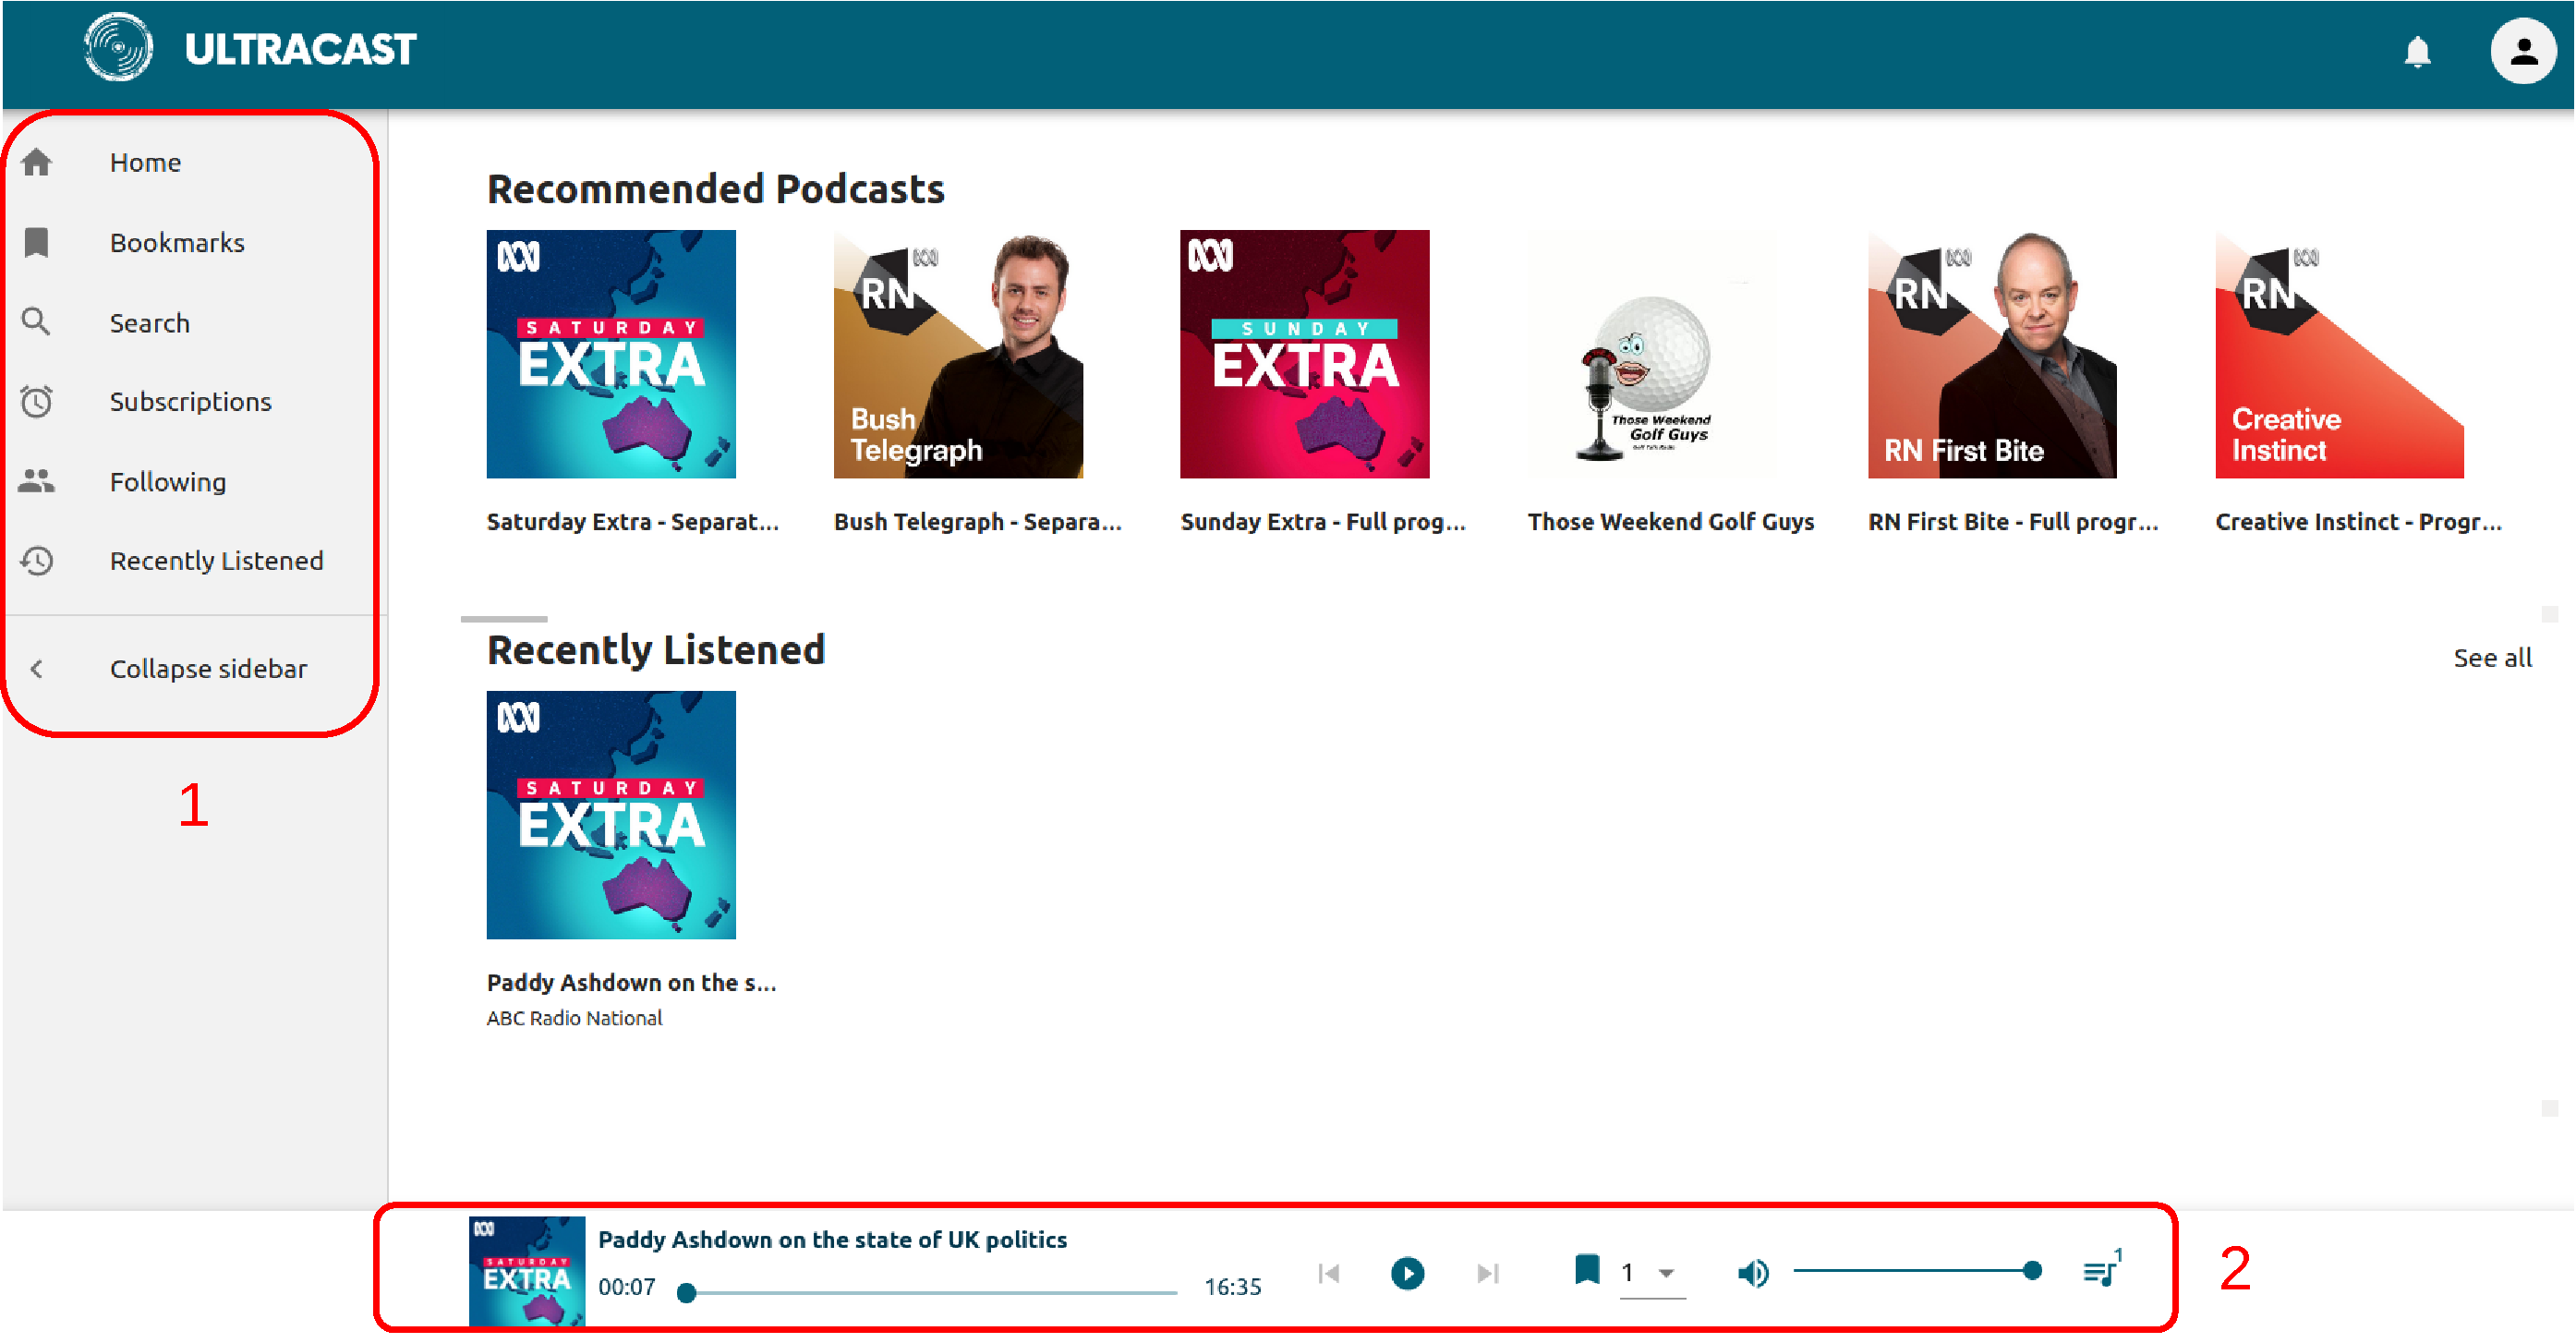
\includegraphics[width=16cm]{resources/UM_Homepage}
    \caption{UltraCast Homepage}
    \label{fig:UM_Homepage} 
\end{figure}

\subsubsection{Searching}

To search for a podcast simply click on "Search" in the pages sidebar and type your search term in the search bar
which will return matching podcasts as seen in \cref{fig:UM_search_result}. Each "tile" in the search result represents
a podcast. The "SAVE SEARCH AS STREAM" button can be used to save a search term. If the search bar is empty then you 
will be able to view and click on a saved "Stream" to apply that search term.

\begin{figure}[ht] 
    \centering
    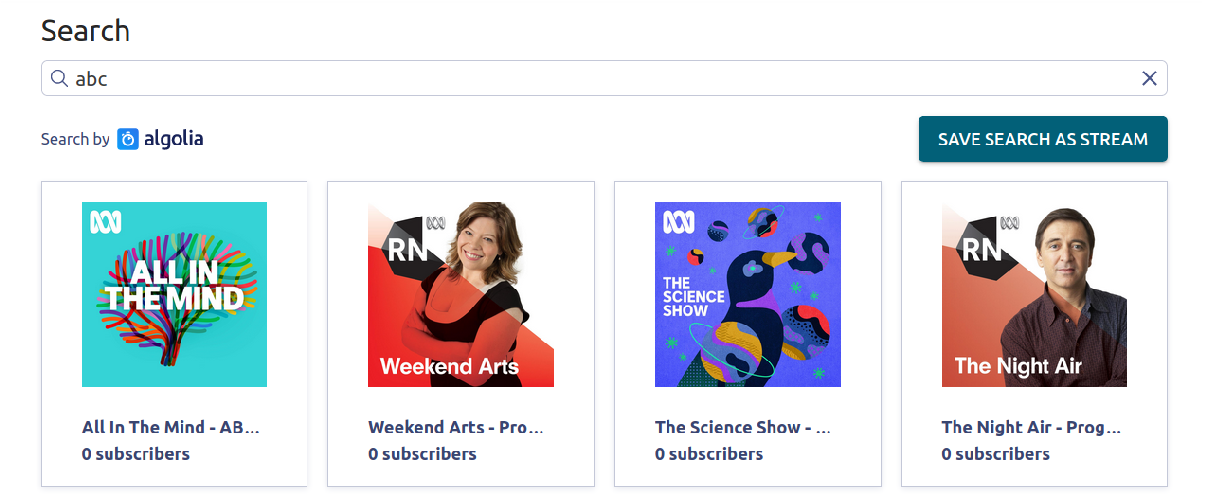
\includegraphics[width=16cm]{resources/UM_Search_Result}
    \caption{UltraCast Search Result}
    \label{fig:UM_search_result} 
\end{figure}

\newpage

%TODO viewing podcasts once it has been clicked on \todo{remove me}
%TODO at what point describe "click on" on the cover art with play button

\subsubsection{Playing Podcast Episodes} \label{sssec:UM_playing_episodes}

Once an episode has been clicked on (via the cover image) it will be added to
the end of a queue in the "Player", which is labelled "8" in \cref{fig:UM_episode_player}.
%
\begin{figure}[ht]
    \centering
    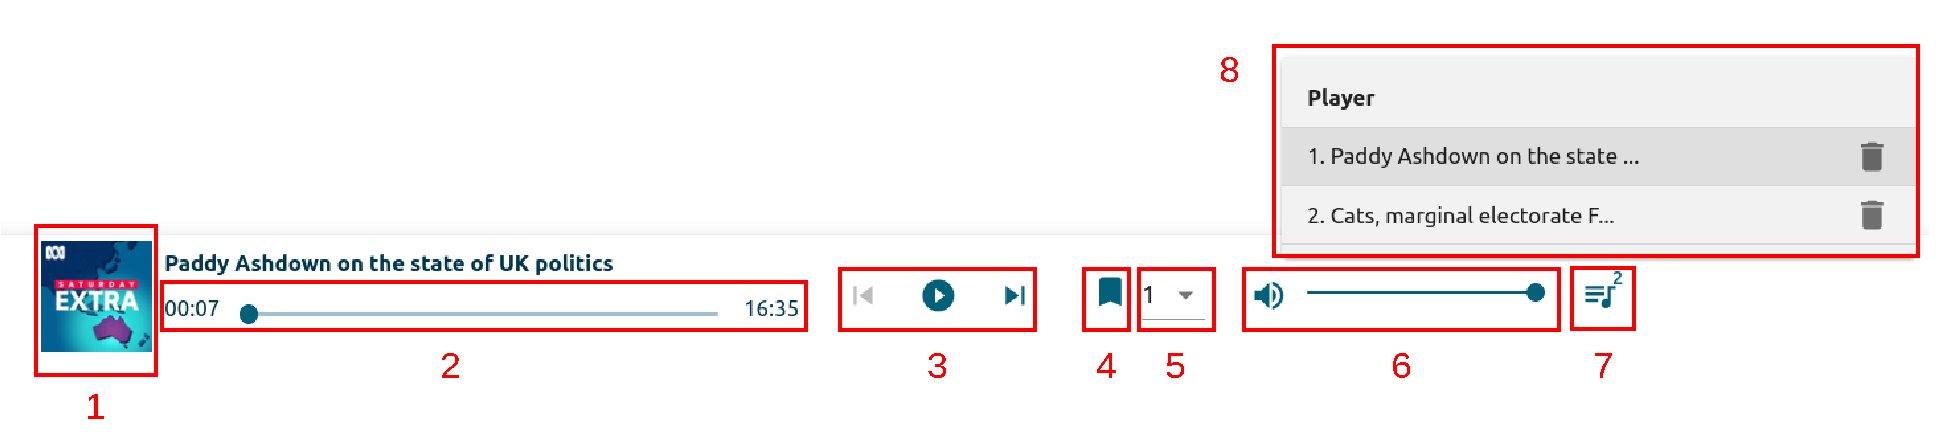
\includegraphics[width=16cm]{resources/UM_Episode_Player}
    \caption{UltraCast Episode Player}
    \label{fig:UM_episode_player} 
\end{figure}
% 
The components of the Episode Player, marked in \cref{fig:UM_episode_player}, are:
\begin{enumerate}
    \item \textbf{Podcast Cover Art} - Click on to view the podcast the episode is part of
    \item \textbf{Episode Audio Track} - Can "pull and drag" to specific timestamp
    \item \textbf{Episode Controller} - Start/pause episode and navigate to next/previous in Player
    \item \textbf{Bookmarks} - Click on to create Bookmark (See \cref{sssec:UM_bookmarks})
    \item \textbf{Playback Speed Control}
    \item \textbf{Volume Control}
    \item \textbf{Player Toggle} - Toggle the Player pop-up on/off
    \item \textbf{Player} - Playlist of episodes. Click on episode in player to start it. Click the bin icon to remove an episode. Player will automatically play the next episode once the current one has ended.
\end{enumerate}

\subsubsection{Bookmarks} \label{sssec:UM_bookmarks}

Bookmarks allow you to create a note which is linked to a timestamp in an episode. To create a bookmark , then fill in the title and description. 
\begin{enumerate}
    \item Click the bookmark icon, 4 in \cref{fig:UM_episode_player}, when you are at the timestamp in the episode that you to mark
    \item Optionally, fill in the title and description in the pop-up
    \item Click the "SAVE" button
\end{enumerate}
%
Bookmarks can be viewed in the Bookmarks page as seen in \cref{fig:UM_bookmark}. The numbered labels are described below:
\begin{enumerate}
    \item Click "Bookmarks" to navigate to the Bookmarks page
    \item Click the drop down to show all the bookmarks for a given episode
    \item Click to play that episode and jump to the saved timestamp
    \item Click to delete the bookmark
\end{enumerate}
\begin{figure}[ht]
    \centering
    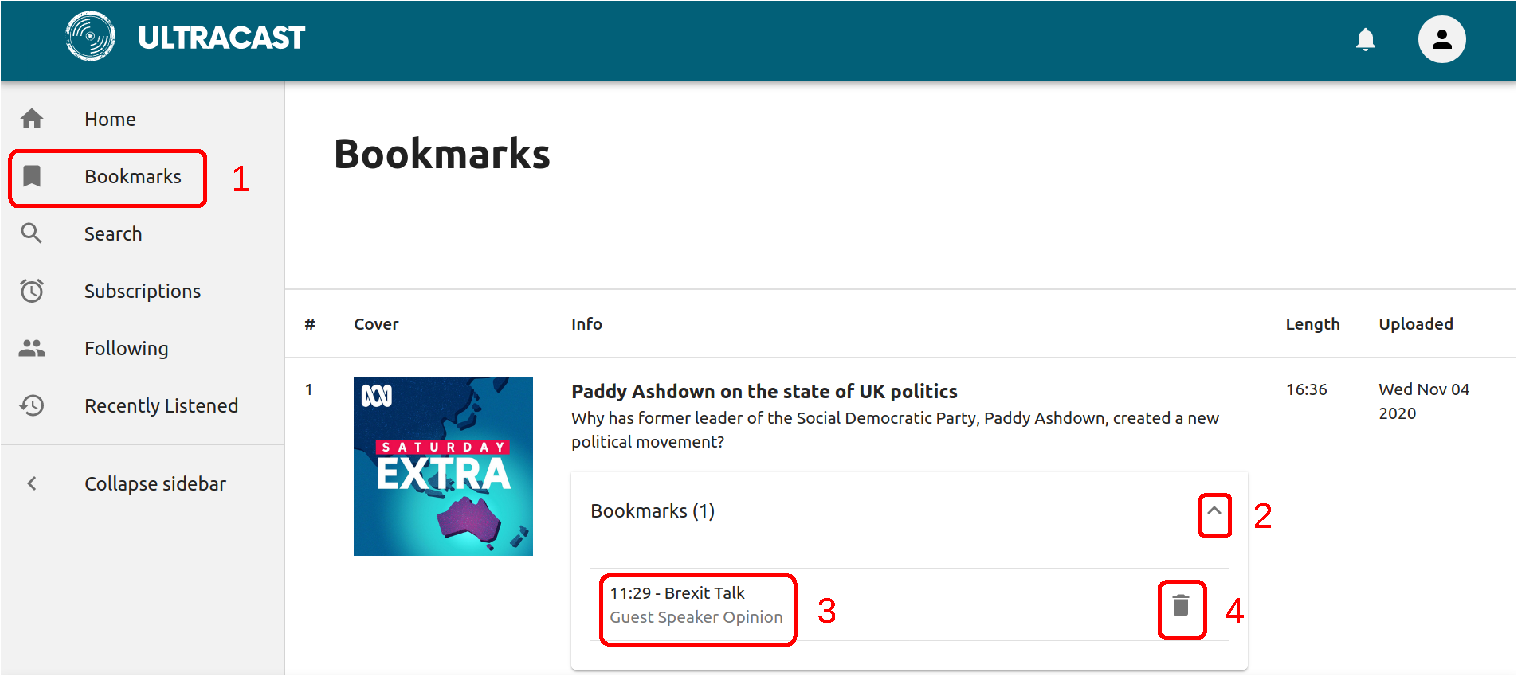
\includegraphics[width=16cm]{resources/UM_Bookmark}
    \caption{UltraCast Bookmark Page}
    \label{fig:UM_bookmark} 
\end{figure}

\newpage

\subsubsection{Creator / Listener Mode and Logging Out} \label{sssec:user_modes}
To logout or swap between creator and listener mode, click on the user icon in the top right corner
which will display the drop down shown in \cref{fig:UM_user_options}.
\begin{figure}[ht]
    \centering
    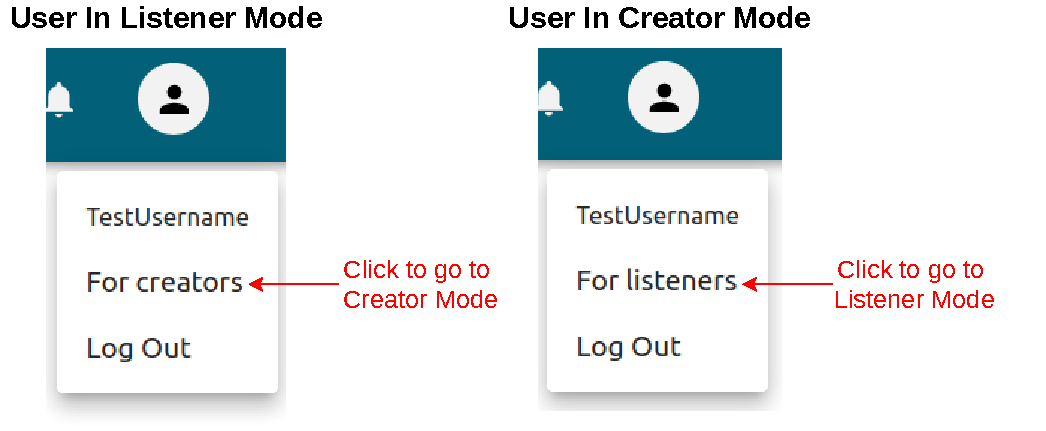
\includegraphics[width=10cm]{resources/UM_CLL}
    \caption{UltraCast User Options}
    \label{fig:UM_user_options} 
\end{figure}

\subsubsection{Creator Mode - Creating Podcasts and Episodes}
Ensure you are in creator mode as described in \cref{sssec:user_modes}. As per \cref{fig:UM_create} to create
a podcast or episode:
\begin{enumerate}
    \item Click "Upload" on the pages sidebar
    \item In the podcast series bar, select "New Podcast" if you wish to create a new podcast or select an existing podcast if you wish to add a new episode
\end{enumerate}
%
From this point you will be guided through the creation process.
\begin{figure}[ht]
    \centering
    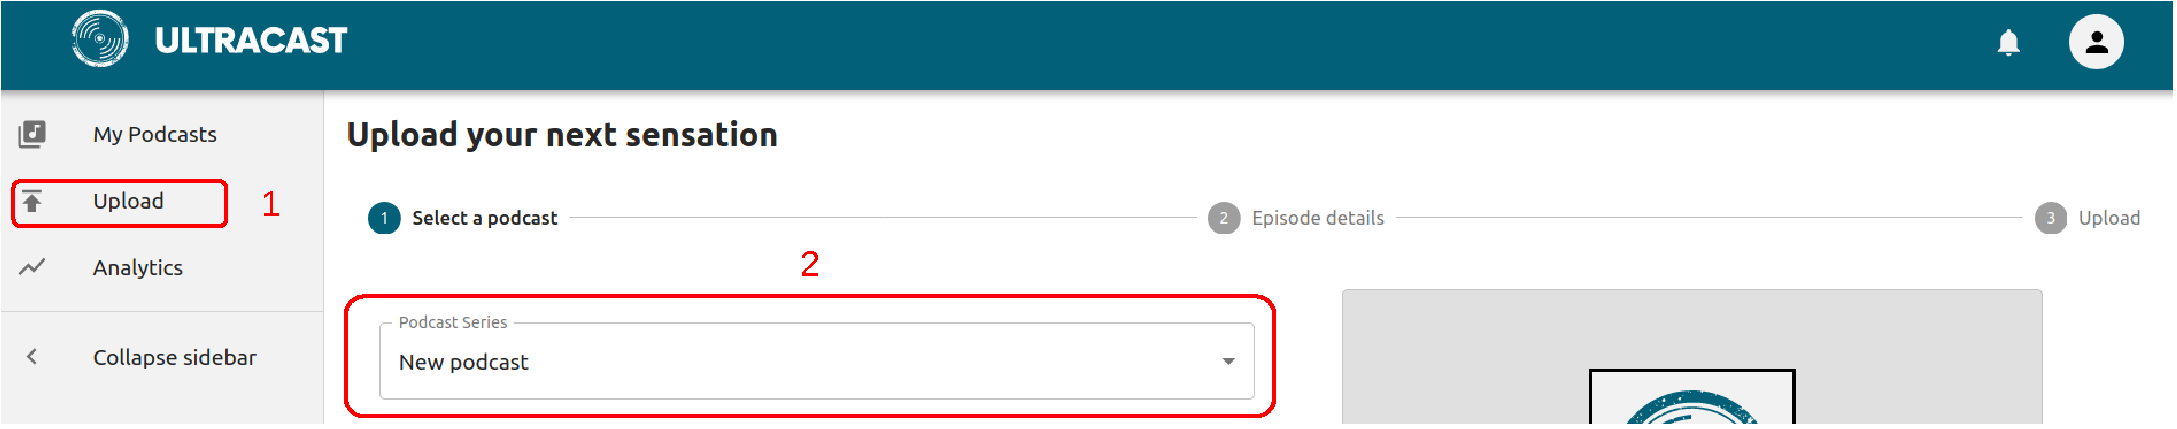
\includegraphics[width=16cm]{resources/UM_Create}
    \caption{UltraCast Create Podcasts and Episodes}
    \label{fig:UM_create} 
\end{figure}

\subsubsection{Creator Mode - Editing Podcasts and Episodes}

Ensure you are in creator mode as described in \cref{sssec:user_modes}. 
To edit a podcast or episode that you have created, as shown in \cref{fig:UM_edit}:
\begin{enumerate}
    \item Click "My Podcasts" on the pages sidebar, then click on the podcast you wish to edit
    \item Use these buttons to edit the podcast
    \item Use these buttons to edit the episode
\end{enumerate}
\begin{figure}[ht]
    \centering
    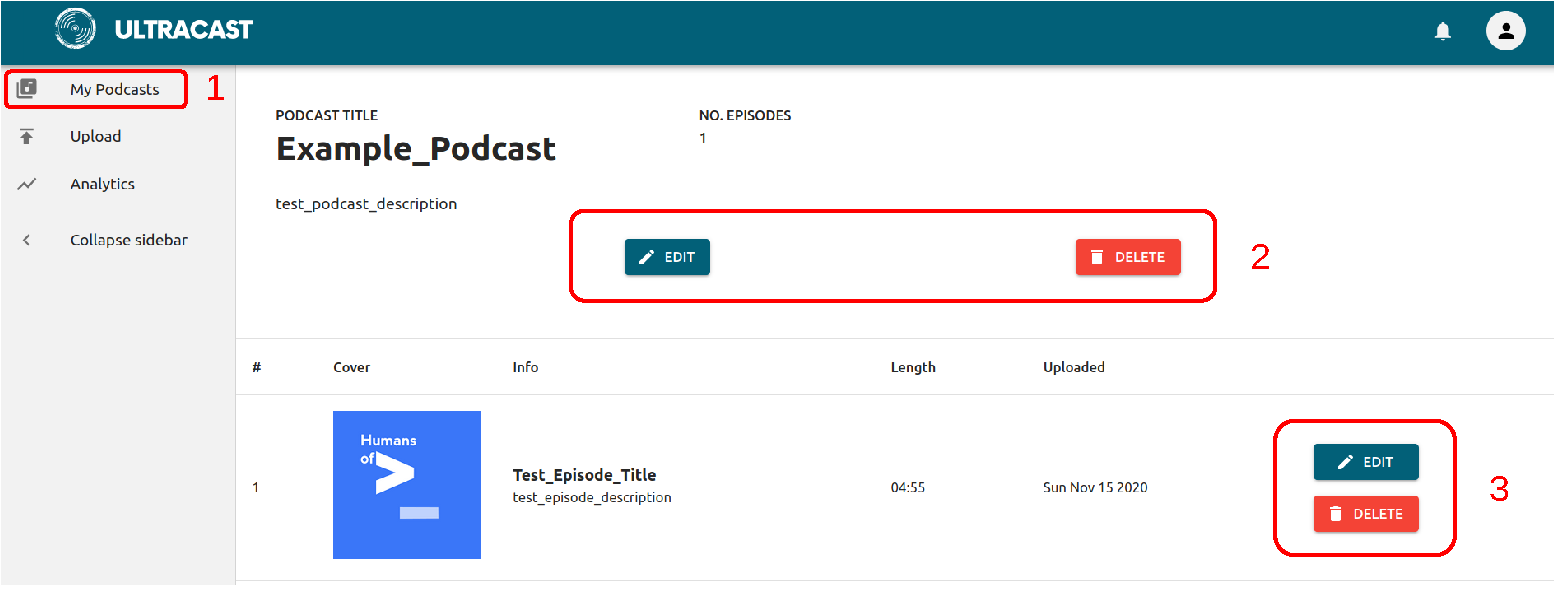
\includegraphics[width=16cm]{resources/UM_Edit}
    \caption{UltraCast Edit Podcasts and Episodes}
    \label{fig:UM_edit} 
\end{figure}

\subsubsection{Creator Mode - Analytics}

Ensure you are in creator mode as described in \cref{sssec:user_modes}.
Creator analytics can be accessed as follows, as shown in \cref{fig:UM_Analytics}:
\begin{enumerate}
    \item Click "Analytics" on the pages sidebar
    \item Click "Overview" to view podcast/episode metrics
    \item Click "Audience" to view a geographical heat-map of viewers
\end{enumerate}
\begin{figure}[ht]
    \centering
    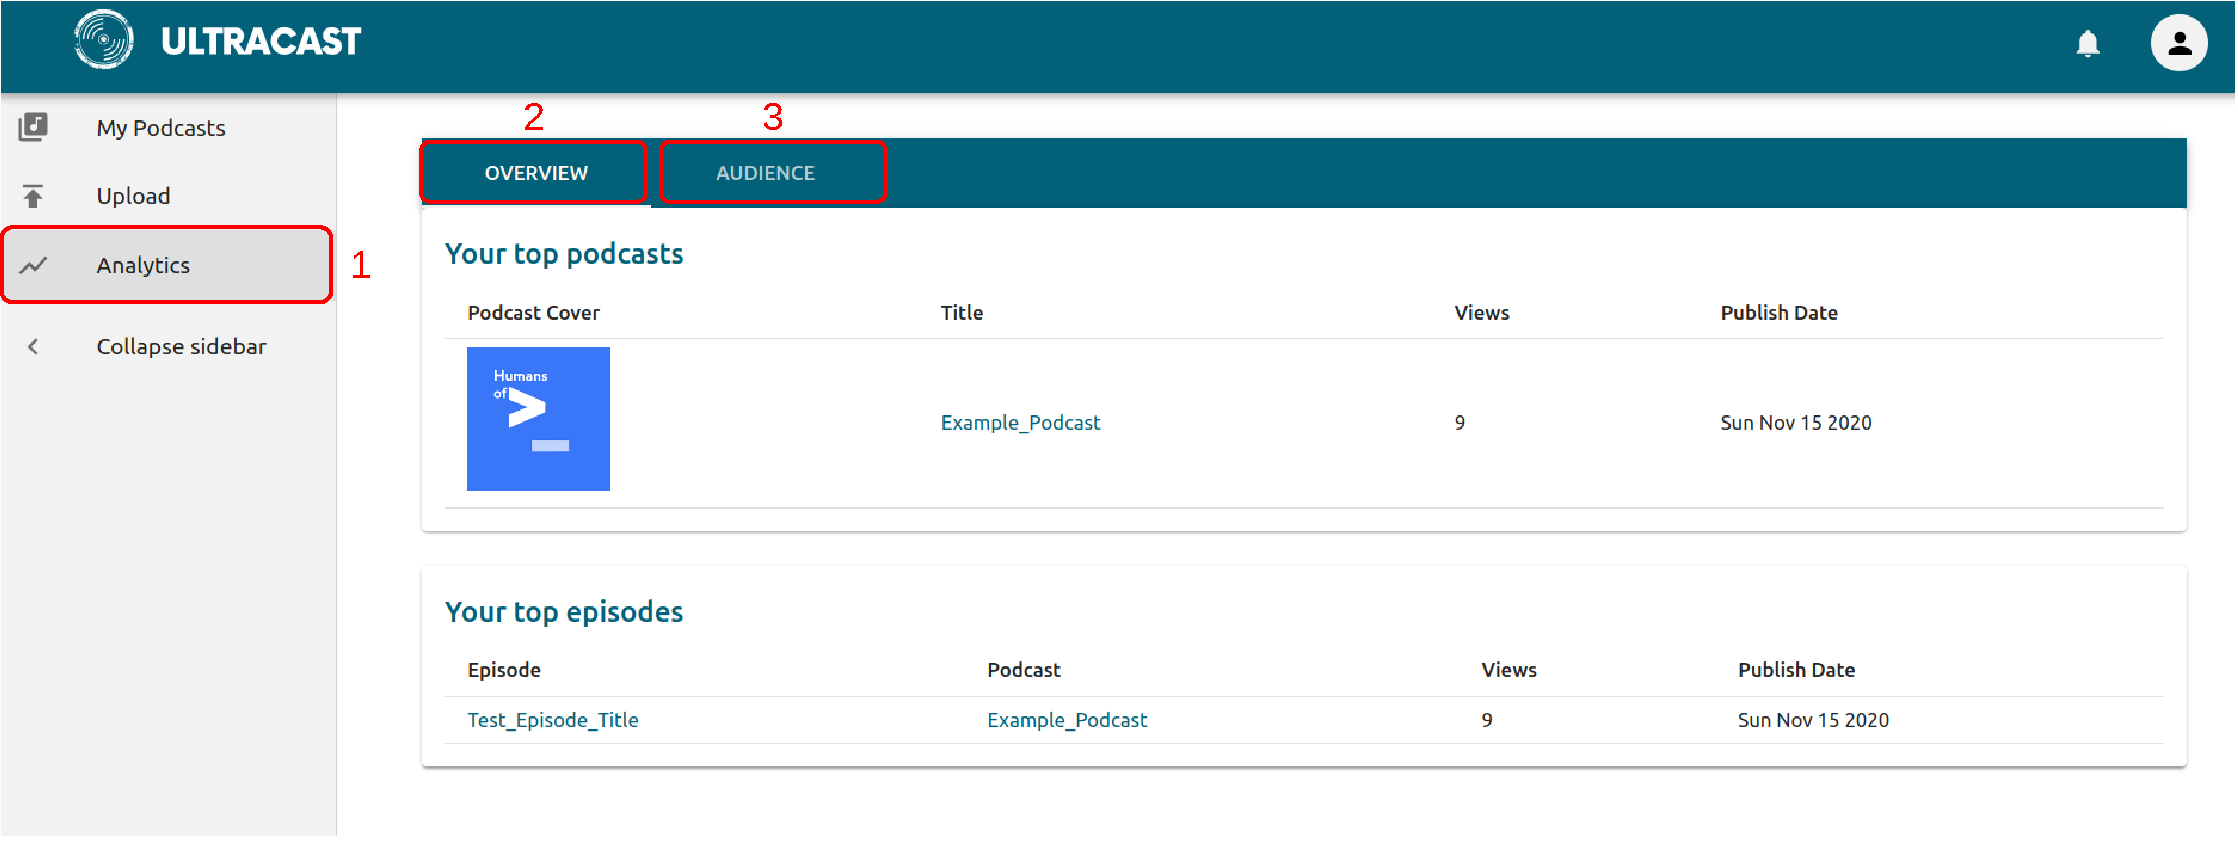
\includegraphics[width=16cm]{resources/UM_Analytics}
    \caption{UltraCast Analytics}
    \label{fig:UM_Analytics} 
\end{figure}

\subsubsection{Subscribing}
To follow another user and view their listen history see the steps below with reference to \cref{fig:UM_subscribe}:
\begin{enumerate}
    \item Click "Subscribe" on a podcast
    \item Click "Subscriptions" on the pages sidebar to view podcasts your are subscribed to
    \item When an episode you are subscribed to uploads a new episode a notification will be displayed on the bell icon
\end{enumerate}
\begin{figure}[ht]
    \centering
    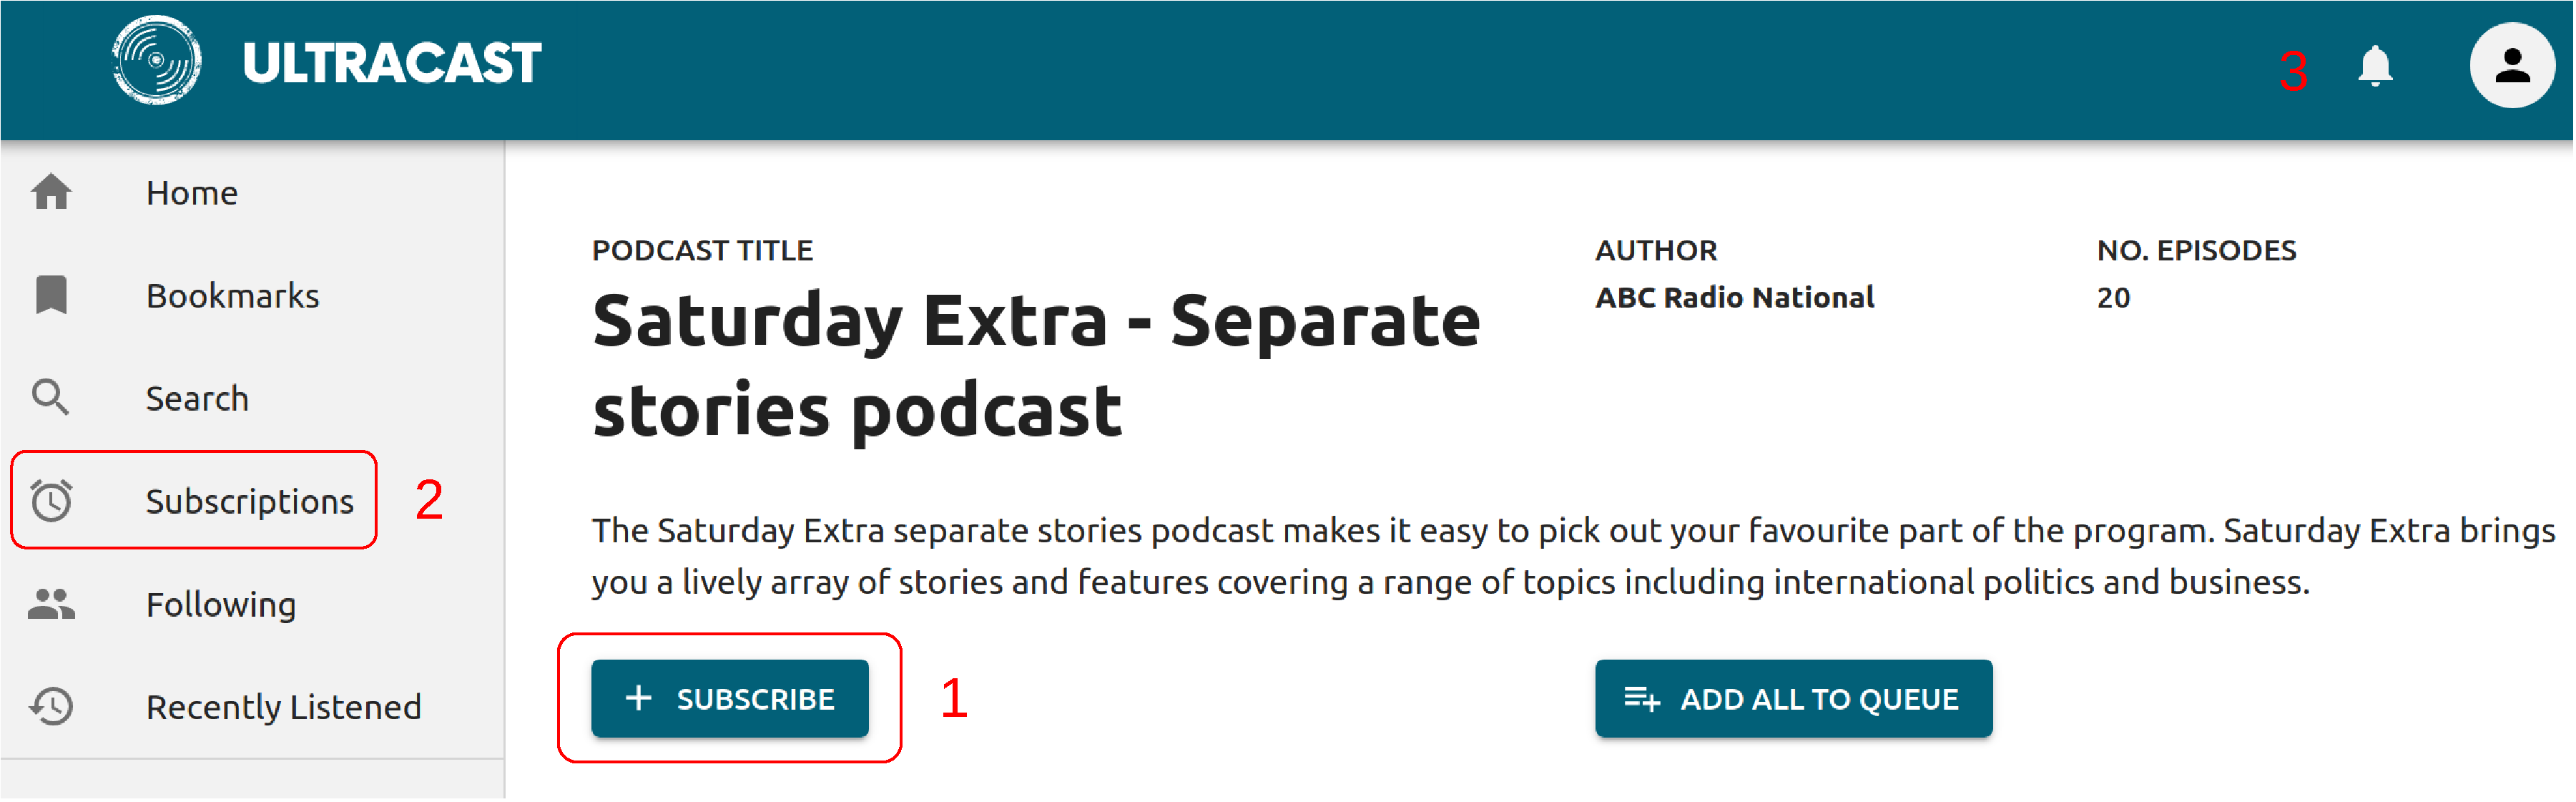
\includegraphics[width=16cm]{resources/UM_Subscribe}
    \caption{UltraCast Subscribing}
    \label{fig:UM_subscribe} 
\end{figure}


\subsubsection{Following}
To follow another user and view their listen history see the steps below with reference to \cref{fig:UM_following}:
\begin{enumerate}
    \item Click "Following" on the pages sidebar
    \item Search user by their email and hit enter
    \item Click "Follow" on that user
\end{enumerate}
\begin{figure}[ht]
    \centering
    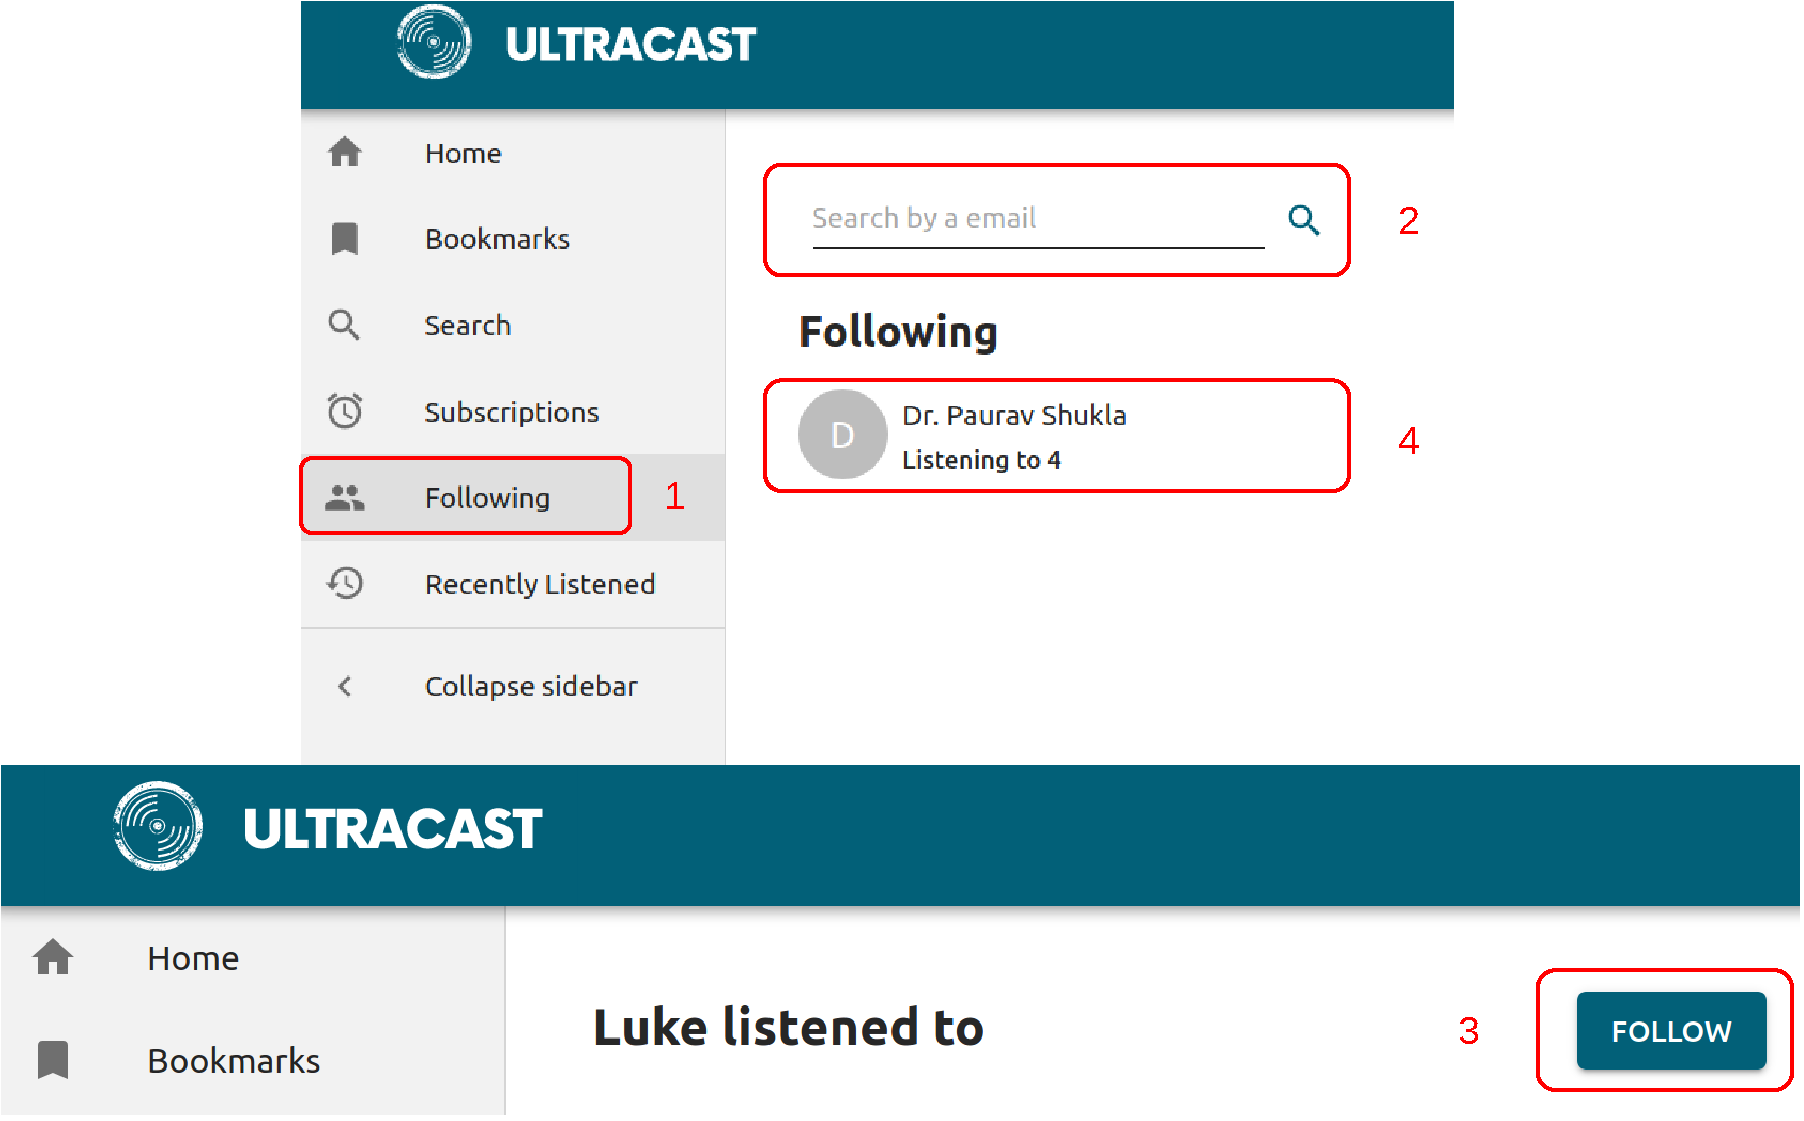
\includegraphics[width=16cm]{resources/UM_Follow}
    \caption{UltraCast Following}
    \label{fig:UM_following} 
\end{figure}

\end{document}

